\chapter{Data generation}\label{ch:method}
In this chapter we will outline how the data needed for the data-driven methods is generated.
This is a crucial step in the process, as the data is used to train the models. 

We will also present the mesh generation for the sphere, which is used to solve the SWE in spherical coordinates.
The data generation is done by solving the SWE in 1D using the FVM with the Godunov scheme and the exact Riemann solver.
We use Gaussian functions with parametric extension~\cite{Gaussian} to generate the initial conditions.


\section{1D SWE: True solution}
In this section, we present how the so-called true solution is found in the code by solving the Riemann problem exactly.
The true solution is found by solving the Riemann problem exact, with 5000 cells, and distinguishing between the wetbed or drybed case, and also identifying the shock and rarefaction waves.
First we caculate the wave speeds for the left and right states, respectively, as
\begin{align*}
    c_L = \sqrt{g h_L}, \quad c_R = \sqrt{g h_R},
\end{align*}
which are used to determine the critical water height $h_{\text{crit}}$ as
\begin{align*}
    h_{\text{crit}} = (u_R - u_L) - 2(c_L + c_R).
\end{align*}
If either $h_L \leq 0$ or $h_R \leq 0$, we are in a drybed case.
If $h_{\text{crit}} \geq 0$ it means the water depth is somehow critical, and we are in a drybed case,
If none of the above conditions are met, we are in a wetbed case.
Summarized:
\begin{align*}
    \begin{cases}
        \text{Dry-bed case} & \text{if }  h_L \leq 0, \quad  h_R \leq 0 \text{ or } h_{\text{crit}} \geq 0, \\
        \text{Wet-bed case} & \text{otherwise}.
    \end{cases}
\end{align*}
For a dry bed case, we then identify where the dry is located, i.e., if the left side is dry, the right side is dry, or the middle is dry, and calculate the wave speeds accordingly.
For a wet bed case, we compute the characteristics $h_*$ and $u_*$ for the star region.
We then identify the shock and rarefaction waves, and calculate the wave speeds for the left and right states, respectively.

FLOW-DIAGRAM.


\section{Data generation}
We use the Matlab script: SWE1D-data-generation to generate the data for the training and testing of the neural network, and the Python script: data-generation to load and visualize the data.
The data generation is done by solving the SWE in 1D using the FVM with the Godunov scheme and the exact Riemann solver.
We use Gaussian functions with parametric extension~\cite{Gaussian} to generate the initial conditions, that is, functions on the form
\begin{align*}
    h(x,0) &= a \exp{\left(\frac{-{(x-\mu)}^2}{2\sigma^2}\right)}, \\
\end{align*}
where $a$ is the amplitude of the Gaussian, $\mu$ is the mean value, and $\sigma$ is the standard deviation.
We solve the 1D SWE with the following parameters:
\begin{itemize}
    \item $N = 200$ cells,
    \item From $t = 0.0$ to $t_{\text{end}} = 1.0$,
    \item $x \in [0, 1]$,
    \item $u(x,0) = 0$,
    \item $b(x) = 0.0$,
    \item $g = 9.81$ and
    \item $\sigma = 0.1$.
\end{itemize}
The value of $\mu$ is varied to generate different initial conditions, as seen in Figure~\ref{fig:data_generation_initial}.
\begin{figure}[H]
    \centering
    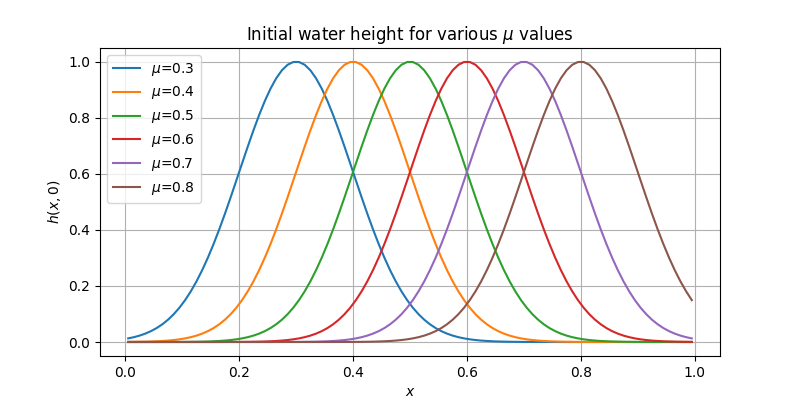
\includegraphics[width=0.8\textwidth]{C:/Users/Matteo/Shallow-Water-Equations/plots/data_generation_initial.png}
    \caption{Initial conditions for the data generation.}\label{fig:data_generation_initial}
\end{figure}


\section{Data Copernicus}

\begin{figure}[H]
    \centering
    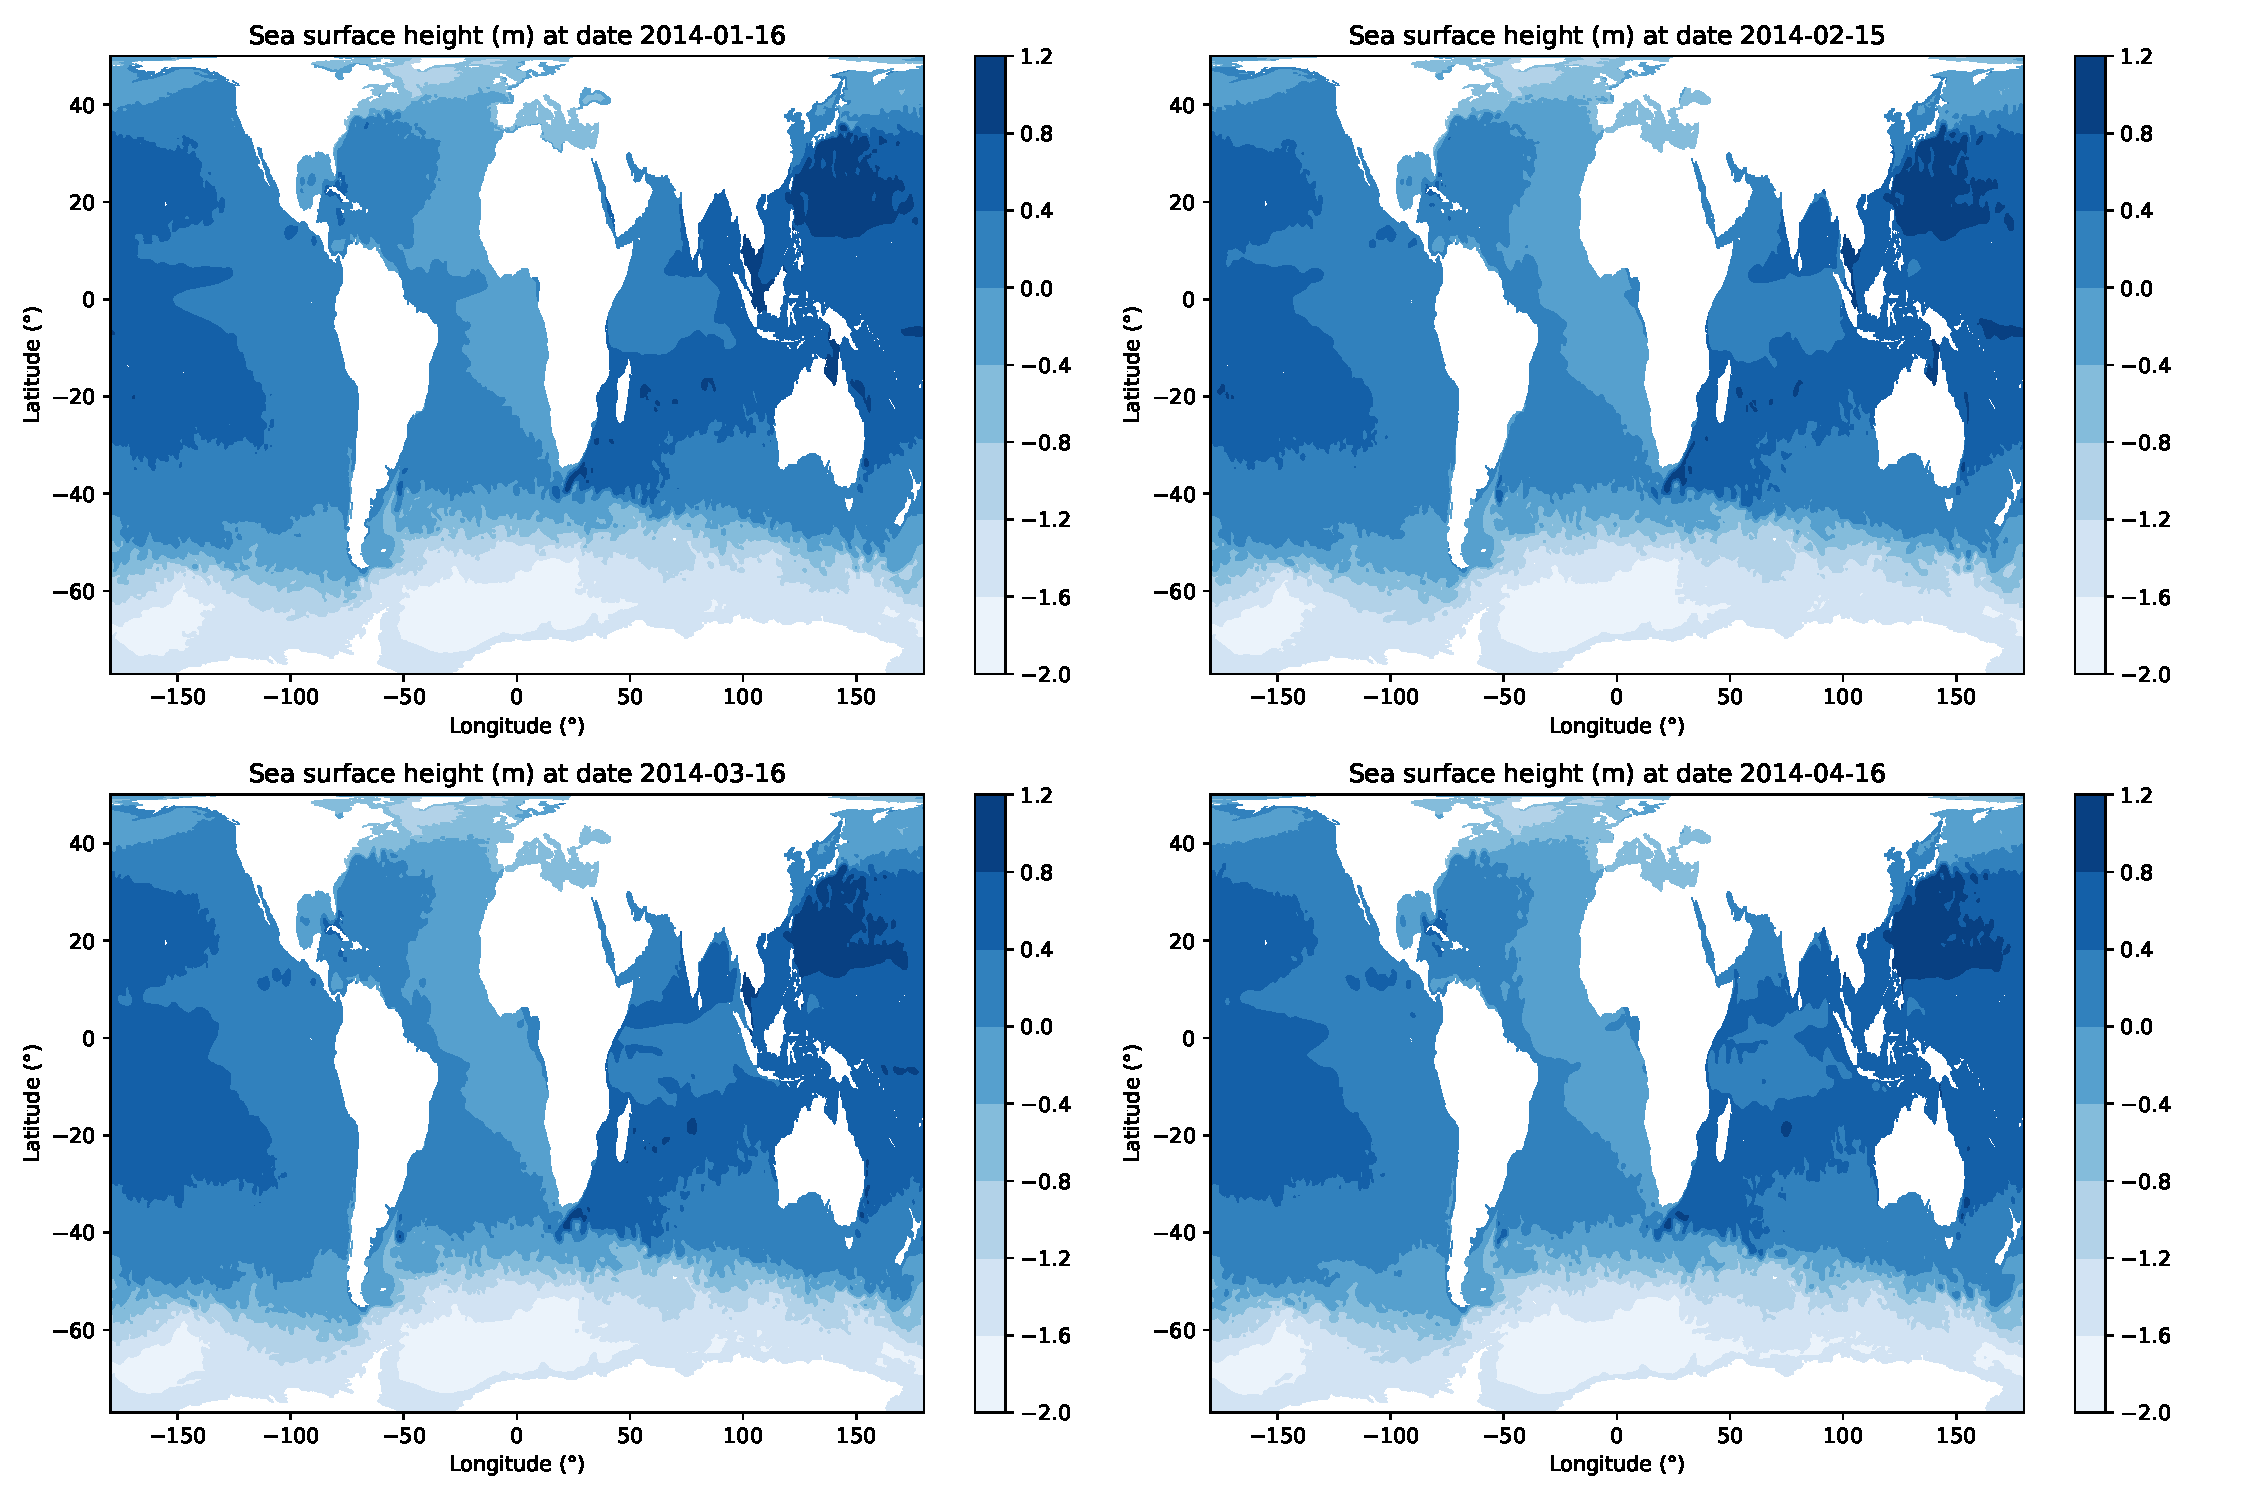
\includegraphics[width=0.95\textwidth]{C:/Users/Matteo/Shallow-Water-Equations/plots/ssh_field.pdf}
    \caption{Sea surfae height as the diffference from reference sea surface height for the months jan-apr 2014.}\label{fig:copernices-ssh}
\end{figure}


\section{Mesh generation for the sphere}
To solve the SWE on the sphere, we must use another grid, than the regular grid used in the 2D case.
Hence, we use the icosahedral grid, which is a grid that approximates the sphere with triangles.
The grid can be generated in different generations, depending on the level of detail we need. 
For each time we refine to a higher level, the number of triangles increases by a factor of four, i.e., we split each triangle into four smaller triangles.
Meaning that the number of triangles is increasing drastically with each level of refinement.
The grid is generated by the Github: https://github.com/siddharth-maddali/SphereMesh/tree/master and then rewritten to Python.
The grid for the first 4 levels of refinement is shown in Figure~\ref{fig:icosahedral_grid}.
\begin{figure}
    \centering
    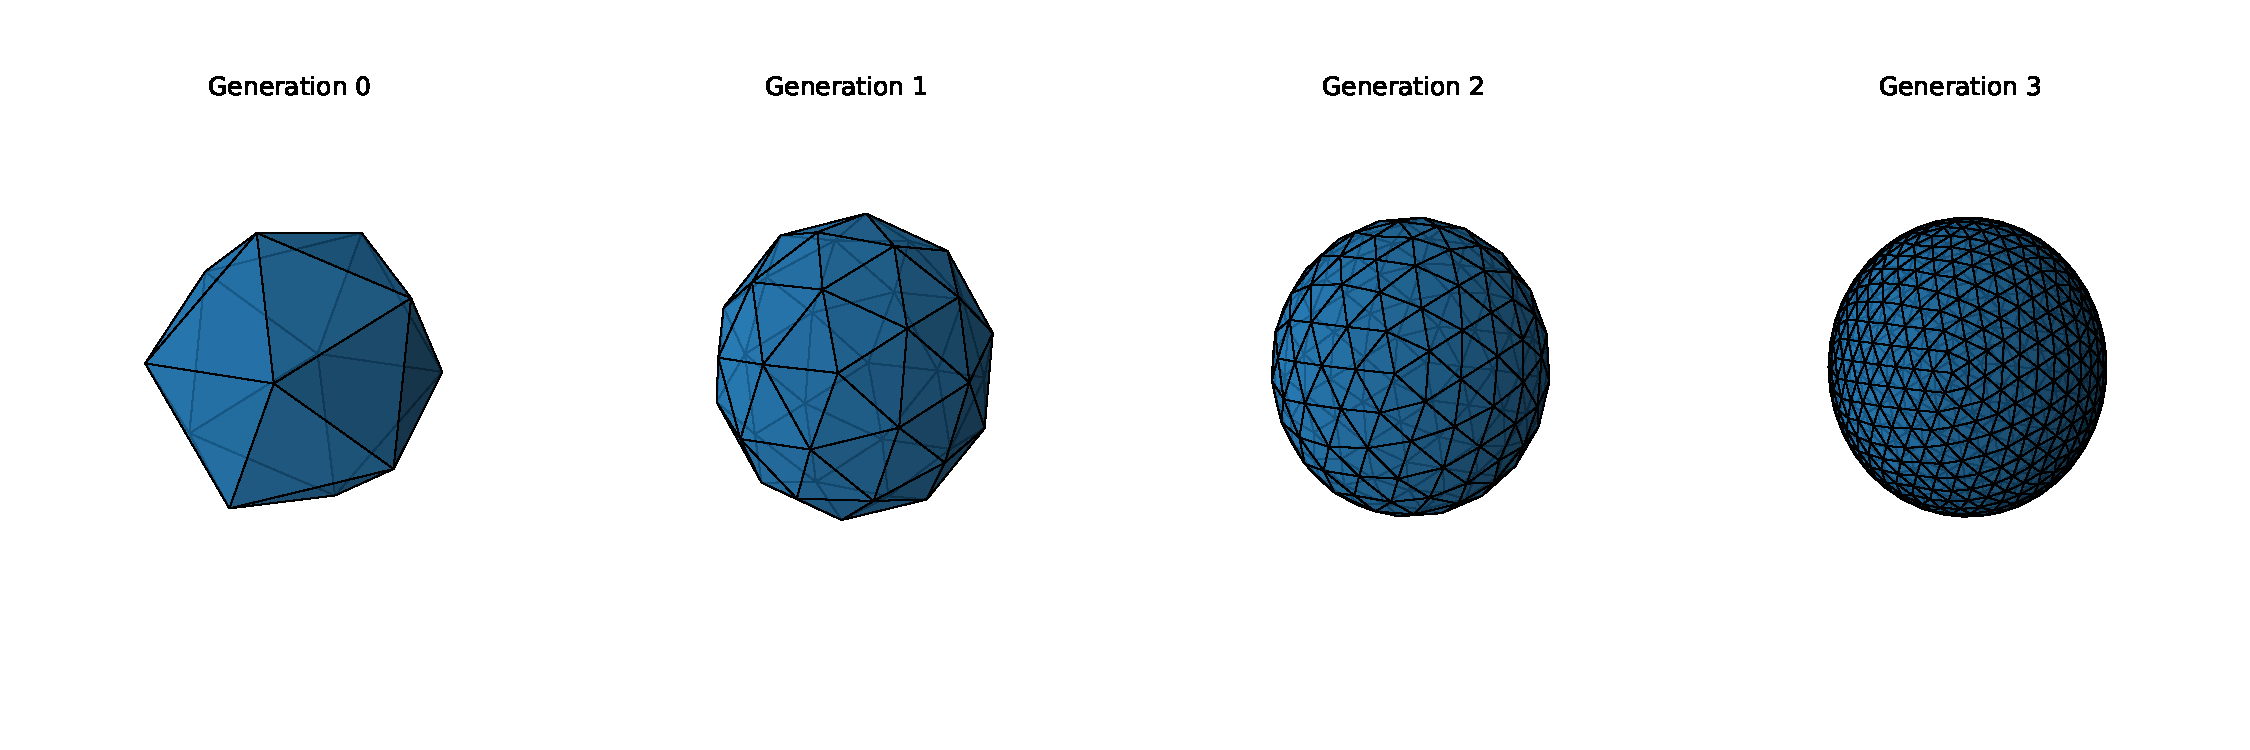
\includegraphics[width=\textwidth]{C:/Users/Matteo/Shallow-Water-Equations/plots/icosahedral_mesh_refinement.pdf}
    \caption{Icosahedral grid for the first 4 levels of refinement.}\label{fig:icosahedral_grid}
\end{figure}
For simplicity, we will begin by considering the first level of refinement, which consists of 20 triangles.
The matrix tri is a $20 \times 3$ matrix, where each row represents a triangle and the three columns represent the three vertices of the triangle.
The vertices are stored in the matrix $P$, which is a $12 \times 3$ matrix, where each row represents a vertex and the three columns represent the x, y, and z coordinates of the vertex.
The vertices are normalized to the unit sphere, i.e., the radius of the sphere is 1.
The idea is now, that similar to the case in cartesian coordinates, we loop through each cell, in this case triangles, and calculate the fluxes between the cells.
We must be aware of which cells/triangles are neighbors, and we must also be aware of the orientation of the triangles, i.e., the normal vector of the triangle.
The normal vector is calculated by the cross product of the two vectors that span the triangle.
The normal vector is then normalized to the unit sphere.
The matrix tri is my Element to Vertex matrix. 
I also need an Element-to-Face table and a Element-to-Element table.
The Element-to-Face table is used to define which edges or faces belong to each triangle.
Each face of a triangle is an edge shared between two triangles.
The Element-to-Element table is used to define which triangles are neighbors. 
That is, it indicates which triangles share an edge. This is important when calculating the fluxes between the triangles.
To construct this table we loop through each triangle and check if the edge of the triangle is shared with another triangle.


We make the FVM to solve SWE for a triangular grid on the sphere.
For each triangle, we consider each face (edge).
For each face we define the normal vector in terms of the spherical unit vectors $\mathbf{e}_\theta$ and $\mathbf{e}_\phi$.
The spherical unit vectors at a point are:
\begin{align*}
    \mathbf{e}_\theta &= \begin{bmatrix}
        - \sin(\theta) \\
        \cos(\theta) \\
        0
    \end{bmatrix}, \\
    \mathbf{e}_\phi &= \begin{bmatrix}
        \cos(\phi) \cos(\theta) \\
        \cos(\phi) \sin(\theta) \\
        -\sin(\phi)
    \end{bmatrix}.
\end{align*}
Where $\mathbf{e}_r$ is the radial direction, going outward from the origin.
$\mathbf{e}_\theta$ is the longitude direction, and $\mathbf{e}_\phi$ is the latitude direction.
The unit vectors are tangensial to the sphere.
We do not need to consider the radial direction, as the SWE is only in the tangential directions.

Now we have the cartesian edge vectors in tangential directions, $\mathbf{e}_0, \mathbf{e}_1, \mathbf{e}_2$.

The projection of an edge vector \( \mathbf{e}_i = (e_{ix}, e_{iy}, e_{iz}) \) onto \( \mathbf{e}_\theta \) is:

\[
\mathbf{e}_i \cdot \mathbf{e}_\theta = e_{ix} \left( -\sin \theta \cos \phi \right) + e_{iy} \left( -\sin \theta \sin \phi \right) + e_{iz} \cos \theta
\]

Similarly, the projection onto \( \mathbf{e}_\phi \) is:

\[
\mathbf{e}_i \cdot \mathbf{e}_\phi = e_{ix} \left( -\sin \phi \right) + e_{iy} \cos \phi
\]

Recall that the cross product between two vectors in 3D produces a third vector that is orthogonal to the two input vectors, i.e., the plane spanned by the two input vectors.

For a given face $f$ of a triangle, we first calculate the Cartesian face normal $\mathbf{n}_f$ as the cross product of the two vectors that span the face.
For a given face $f$ of a triangle, we define the normal vector $\mathbf{n}_f$ is decomposed into the spherical unit vectors as


